% AI-Intent: Conceptual Modeling for Accountable Multi-Agent AI Systems
% Springer LNCS format for ER 2026 (Conceptual Modeling Conference)

\documentclass[runningheads]{llncs}

\usepackage[T1]{fontenc}
\usepackage{graphicx}
\usepackage{booktabs}
\usepackage{amsmath}
\usepackage{amssymb}
\usepackage{listings}
\usepackage{xcolor}
\usepackage{hyperref}
\usepackage{tikz}
\usepackage{multirow}
\usetikzlibrary{arrows.meta, positioning, shapes.geometric, fit}
\usepackage{comment}
\usepackage{tabularx}
\usepackage{tablefootnote}
\usepackage{soul}
\sethlcolor{yellow}

\lstset{
  basicstyle=\ttfamily\small,
  keywordstyle=\color{blue}\bfseries,
  stringstyle=\color{red!70!black},
  commentstyle=\color{green!50!black}\itshape,
  breaklines=true,
  frame=single,
  numbers=left,
  numberstyle=\tiny\color{gray},
  backgroundcolor=\color{gray!5},
  captionpos=b,
  aboveskip=8pt,
  belowskip=8pt,
}

\begin{document}

\title{AI-Intent: A Conceptual Modeling Framework\\
for Accountable Multi-Agent AI Systems}

\titlerunning{AI-Intent: A Conceptual Modeling Framework}

\author{Wolfgang Maass\inst{1} \and Iris Reinhartz-Berger\inst{2}}
\authorrunning{W.~Maass{} and I.~Reinhartz-Berger}
\institute{German Research Center for Artificial Intelligence (DFKI)\\
and Saarland University, Saarbr\"ucken, Germany\\
\email{wolfgang.maass@dfki.de}
\and University of Haifa, Haifa, Israel\\
\email{iris@is.haifa.ac.il}}

\maketitle

\begin{abstract}
Existing agent-oriented conceptual modeling frameworks assume components with deterministic execution semantics. Applied to language model agents, whose outputs arise from probabilistic text generation governed by natural-language inputs, they lack three constructs that accountability requires: a binary \emph{declaration} of each agent's legitimate action space; runtime \emph{enforcement} of negative obligations by a component external to the agent; and treatment of inter-agent communication as \emph{auditable evidence}.

To address these gaps, we introduce \textsc{AI-Intent},
a conceptual modeling framework organized into three pillars:
\textbf{\textit{Declaration}} encodes each agent's action boundary, decision rights, capabilities, and risk policies in \textit{Mandates}; \textbf{\textit{Enforcement}} evaluates every \textit{Proposed Action} against the applicable \textit{Mandate} through a \textit{Compliance Agent} before delivery; \textbf{\textit{Auditability}} derives a structured, durable \textit{Accountability Trace} from every session.
A reference implementation for private investment advisory under MiFID~II is evaluated across 190 evaluation sessions: boundary violation containment averaged 97.9\% with zero forced-pass occurrences, while audit trace completeness was found to depend on the instruction-following capability of the deployed model.

\keywords{Multi-Agent Systems \and Conceptual Modeling \and
Language Model Agents \and Accountability \and Governance}
\end{abstract}

%=====================================================================
\section{Introduction}
\label{sec:introduction}
%=====================================================================

Language model-based agents are rapidly moving from research prototypes to production systems that support consequential decisions in finance, healthcare, and enterprise operations~\cite{wang2024survey,xi2023rise}.
Unlike traditional software components, whose runtime behavior is fully determined by source code, they generate outputs through probabilistic text generation governed by natural language inputs, training data, and model parameters. When multiple such agents collaborate on joint recommendations, questions arise that existing conceptual models cannot answer: what each agent was supposed to do, whether it stayed within its scope, and why a particular output was produced.

Conceptual modeling frameworks for multi-agent systems have a rich history~\cite{yu2011social,bresciani2004tropos,wooldridge2000gaia}, modeling agents in terms of goals, capabilities, roles, and inter-agent dependencies. These frameworks share an assumption that their components have deterministic or rule-governed execution semantics -- an assumption that does not hold for language model agents, giving rise to three gaps.

%\medskip
\textbf{Gap~1: Intent boundary versus goal satisfaction.}
Traditional goal models, such as $i^*$ and Tropos, treat goal satisfaction as graded~\cite{yu2011social}. For language model agents, the relevant construct is instead a binary \emph{sortal boundary}: a request either falls within the agent's legitimate scope or it does not. An equity analyst agent recommending gold at 35\% allocation has not partially satisfied its goal; it has transgressed its mandate scope.

%\medskip
\textbf{Gap~2: Negative obligations as runtime-enforceable constraints.} Normative frameworks and deontic logic provide well-developed accounts of obligation, permission, and prohibition~\cite{vonwright1951essay,governatori2007characterising,boella2006introduction}, but assume agents that deliberate over norms before acting~\cite{dignum1999autonomous}. Language model agents may acknowledge a constraint and then violate it, or construct superficially plausible justifications for exceptions~\cite{huang2023selfcorrect}. The modeling challenge is therefore to represent negative obligations in a form an \emph{external} enforcement component can evaluate, rather than relying on agent self-compliance.

%\medskip
\textbf{Gap~3: Communication as audit evidence.} Existing agent communication models, such as FIPA-ACL~\cite{fipa2002}, specify message syntax and semantics but treat communication logs as an optional engineering concern. Regulatory frameworks for AI systems, e.g., the EU AI Act~\cite{euaiact2024} and MiFID~II~\cite{mifid2014}, require that every consequential decision be traceable to its inputs -- making communication logging a \emph{structural property} of the conceptual model, not an add-on.

%\medskip
To address these gaps, we propose \textsc{AI-Intent}, with one pillar per gap. \textbf{\textit{Declaration}} introduces the \textit{Mandate}, a first-class artifact encoding an agent's binary action boundary, decision rights, capabilities, and risk policies. \textbf{\textit{Enforcement}} introduces \textit{Intent Enforcement}, a mandatory gatekeeper that evaluates every \textit{Proposed Action} against the applicable \textit{Mandate} and produces a \textit{Compliance Verdict} before delivery. \textbf{\textit{Auditability}} derives an \textit{Accountability Trace} from the \textit{Log Entry} of every verdict. \textcolor{black}{It is important to note that \textsc{AI-Intent} is not a new modeling language, nor a syntactic extension of an existing one; it is a domain-independent \emph{conceptual model}, comprising governance constructs, their metamodel relationships, and well-formedness constraints.
Grounded in the Unified Foundational Ontology (UFO)~\cite{guizzardi2005ontological} and rendered in OntoUML, \textsc{AI-Intent} is intended to \textit{augment} existing agent-oriented languages. }
For evaluating \textsc{AI-Intent}, we developed a reference implementation for private investment advisory. The reference implementation shows that even under a neutral disposition, agents violate their allocation cap on the first attempt often enough to motivate external enforcement as a structural modeling requirement.
%Across 190 sessions, including adversarial disposition presets, boundary violation containment averaged 97.9\% with zero forced-pass occurrences; yet even under a neutral preset, the materials agent violated its allocation cap on the first attempt in 12.9\% of sessions, motivating external enforcement as a structural modeling requirement.
%rather than an engineering convenience.

%\vspace{-1pt}
The remainder of the paper is organized as follows. Section~\ref{sec:background}
reviews existing agent-oriented modeling frameworks. Section~\ref{sec:framework}
presents the \textsc{AI-Intent} framework across its three pillars. Section~\ref{sec:evaluation}
reports the empirical evaluation, while Section~\ref{sec:discussion}
discusses the results. Section~\ref{sec:conclusion} concludes and
identifies directions for future work.

%=====================================================================
\section{Background and Related Work}
\label{sec:background}
%=====================================================================

\textcolor{black}{We scope our review to work proposing modeling constructs for agent governance (Section~\ref{sec:aomodeling}); multi-agent implementation frameworks (Section~\ref{sec:mala}) and AI-governance policy work (Section~\ref{sec:aigov}) serve as deployment substrate and normative context.}

\subsection{Agent-Oriented Conceptual Modeling}
\label{sec:aomodeling}

\textcolor{black}{Four influential modeling approaches are examined through the lens of the three gaps: the goal-oriented $i^*$~\cite{yu2011social} and Tropos~\cite{bresciani2004tropos}, and the more strictly agent-oriented GAIA~\cite{wooldridge2000gaia} and NMAS~\cite{boella2006introduction}. We group them because each supplies constructs that a governance model must either reuse or replace.}

\textbf{The $i^*$ framework}~\cite{yu2011social} models actors with goals, tasks, resources, and softgoals connected by contribution links; its softgoal construct explicitly supports partial satisfaction, a graded semantics well suited to design trade-offs, but inappropriate for mandate boundaries, where violations are categorical rather than a matter of degree.
\textbf{Tropos}~\cite{bresciani2004tropos} extends $i^*$ into a full
development methodology, but likewise provides no construct for prohibitions: both specify what agents can and should do, not what they
must not do.

\textbf{GAIA}~\cite{wooldridge2000gaia} provides role models with permissions, responsibilities, activities, and protocols. Its permission construct is the closest existing analog to boundary constraints: a
role's permissions define the actions it is authorized to take. However, permissions are granted at modeling time and assumed to hold at runtime; no mechanism verifies that an agent stays within them during execution. 
\textbf{Normative Multi-Agent Systems~(NMAS)}~\cite{governatori2007characterising,boella2006introduction,dignum1999autonomous} address obligation and prohibition directly~\cite{vonwright1951essay}, and defeasible deontic logic~\cite{governatori2007characterising} further allows norms to have exceptions and
be defeated by stronger norms. These approaches, however, assume agents that
deliberate over norms before acting -- an assumption that fails for language model agents, whose compliance depends on how norms are represented in the input specification and how reliably the model follows instructions~\cite{huang2023selfcorrect}.

Table~\ref{tab:comparison} summarizes the extent to which the four modeling frameworks cover the identified gaps: $i^*$ and Tropos represent neither prohibitions nor scope boundaries; GAIA adds permissions but cannot verify them at runtime; NMAS closes the representational gap on prohibitions but relies on agent self-deliberation for enforcement, an
assumption that fails for non-deterministic generators. 
%\textcolor{black}{The recent trustworthy-agent frameworks supply runtime auditing and provenance but no declarative modeling constructs for scope, prohibition, or risk. Only AI-Intent covers all eight capabilities, which is the gap the framework is designed to close.}

%\vspace{-14pt}

\begin{table}
\centering
\caption{Comparative analysis of agent governance modeling capabilities across the four agent-oriented modeling frameworks 
%and the recent runtime trustworthy-agent frameworks (Trust.\ MAS: Alqithami's AAF~\cite{alqithami2025adaptive}, verifiability-first agents~\cite{gupta2025verifiability}) with AI-Intent. 
\checkmark~= fully expressible; $\circ$~= partial/with significant extensions; $\times$~=
not expressible without framework revision.}
%Trust.\ MAS are runtime mechanisms, not modeling languages; marks reflect what each represents as an explicit construct. \emph{Model operativity} denotes runtime injection of mandate constraints into the deployed model's input specification.}
\label{tab:comparison}
\setlength{\tabcolsep}{4pt}
\small
%\resizebox{\textwidth}{!}{%
\begin{tabular}{@{}lcccccc@{}}
\toprule
\textbf{Capability} & \textbf{$i^*$} & \textbf{Tropos} &
\textbf{GAIA} & \textbf{NMAS} \\
\midrule
Intent scope (binary sortal boundary) & $\times$ & $\times$ &
    $\circ$ & $\circ$ \\
Negative obligations (prohibitions)   & $\times$ & $\times$ &
    $\circ$ & \checkmark \\
Quantitative risk parameters & $\times$ & $\times$ & $\times$ & $\circ$ \\
Runtime constraint enforcement & $\times$ & $\times$ & $\times$ & $\circ$ \\
External Compliance Agent & $\times$ & $\times$ & $\times$ & $\times$ \\
Audit-native communication & $\times$ & $\times$ & $\times$ & $\times$ \\
Compliance history in trace & $\times$ & $\times$ & $\times$ & $\times$ \\
Model operativity (runtime injection) & $\times$ & $\times$ & $\times$ & $\times$ \\
\bottomrule
\end{tabular}%
%}
\end{table}

%\vspace{-20pt}

\subsection{Multi-Agent Implementation Frameworks}
\label{sec:mala}

Where agent-oriented modeling frameworks lack runtime enforcement, current multi-agent language model architectures lack formal modeling altogether:  AutoGen~\cite{wu2023autogen}, CrewAI~\cite{crewai2024}, and
LangGraph~\cite{langgraph2024} represent agent roles as natural-language descriptions with no formal constraint semantics or runtime verification. The Model Context Protocol
(MCP)~\cite{anthropic2024mcp} standardizes communication between language model applications and external tools, providing interoperability but not governance. 
%AI-Intent builds on MCP's communication substrate and adds the governance layer that MCP lacks.

Output filtering systems, such as NeMo Guardrails~\cite{rebedea2023nemo} and Constitutional AI~\cite{bai2022constitutional}, enforce constraints on single-agent outputs through filtering and self-assessment, but do not model inter-agent accountability: they cannot trace a multi-agent decision to its constituent sub-agent outputs or produce
structured audit artifacts. 
%AI-Intent shares the underlying motivation, namely constraint enforcement on non-deterministic outputs, but operates at the multi-agent communication level rather than at the single-model output level.

\subsection{AI Governance and Accountability}
\label{sec:aigov}

Existing accountability frameworks address individual model decisions~\cite{arrieta2020explainable} and dataset documentation~\cite{gebru2021datasheets,mitchell2019model}, but not \emph{multi-agent accountability}: tracing a joint decision back to the sub-agent outputs and constraint evaluations that produced it. The EU AI Act~\cite{euaiact2024} and MiFID~II mandate transparency and traceability for high-risk and financial AI systems, respectively, but neither specifies how traceability is to be achieved when a decision is the product of multiple
collaborating agents.

\textcolor{black}{A recent line of work targets trustworthiness and accountability in language model agent systems directly. Alqithami's Adaptive Accountability Framework~\cite{alqithami2025adaptive} records verifiable interaction provenance and attributes responsibility via a causal influence graph, targeting \emph{emergent} norm violations at scale; verifiability-first designs~\cite{gupta2025verifiability} embed lightweight audit agents and attestations to minimize time-to-detect misalignment; and governance frameworks for multi-agent AI~\cite{pujari2024ethical,bamil2026unified,am2026self} treat accountability failures as governance-design problems,  proposing evaluation and policy scaffolding. These works 
%share AI-Intent's motivation but differ in level: they 
are runtime, policy, or evaluation \emph{mechanisms}  that detect or attribute violations a posteriori from observed traces.}
%, whereas AI-Intent is a \emph{conceptual model} that specifies the constructs such mechanisms leave implicit -- a declared per-agent action boundary, an external enforcement role, and an audit artifact derived as a well-formedness condition. Where they detect or attribute violations \emph{a posteriori} from observed traces, AI-Intent's enforcement intercepts each Proposed Action \emph{before} delivery. The directions are complementary: a system could realize AI-Intent's constructs and adopt~\cite{alqithami2025adaptive}'s attribution for residual emergent behaviors that per-message enforcement does not cover.}

%Enterprise architecture standards and Service-Oriented Architecture compliance logging provide audit trails as infrastructure services. By design, such logs record what happened; they are not first-class elements that constrain system behavior at runtime. AI-Intent addresses this distinction: in \textit{AI-Intent}, the \textit{Accountability Trace} is a structural model component whose existence is a well-formedness condition, and the \textit{Compliance Verdict} attached to each message is a metamodel relationship rather than a log entry.

%=====================================================================
\section{The AI-Intent Framework}
\label{sec:framework}
%=====================================================================

\textcolor{black}{The analysis of the literature in Section 2 leaves specific gaps: no modeling framework combines declared scope boundaries, enforceable prohibitions, and audit-native communication, and the recent trustworthy-agent line supplies runtime mechanisms without the modeling constructs beneath them. \textsc{AI-Intent} closes these as a metamodel of governance constructs, their relationships, and well-formedness conditions, independent of any implementation. Section~\ref{sec:ontology} states its ontological commitments; Section~\ref{sec:pillars} presents the constructs, distinguishing UFO-derived constructs from design choices layered on top.}

\subsection{Core Principles and Ontological Commitments}
\label{sec:ontology}

\textsc{AI-Intent} uses UFO~\cite{guizzardi2005ontological} and
standard deontic
semantics~\cite{vonwright1951essay,governatori2007characterising} as follows. %\textcolor{black}{We note, however, that the dependence on UFO is for ontological categorization of \textsc{AI-Intent}'s constructs, not for its runtime operation: a deployment operationalizes these categories without ontological inference.}

\textbf{Agents as intentional objects.} Agents are UFO intentional objects with dispositions to act; a Mandate specifies the intended disposition -- the behaviors the agent is authorized to exhibit and the boundaries it must not cross. This lets the Mandate constrain a disposition-to-act rather than only observed behavior.
%and the risk parameters within which it must operate.

\textcolor{black}{\textbf{Intent scope as a sortal boundary.} We use \emph{sortal} in its
established ontological sense: a sortal universal supplies a principle of identity and individuation, determining for any candidate whether it \emph{is or is not} an instance of the type~\cite{guizzardi2005ontological}, and is therefore inherently binary rather than graded. The intent scope in the Mandate is accordingly not a goal admitting degrees of satisfaction, but a natural-language specification of such a boundary, whose identity criterion makes ``the same kind of request'' well defined across the paraphrastic variation typical of language model queries.}

\textbf{Boundary constraints as prohibitions.} Following deontic logic~\cite{vonwright1951essay}, the boundary constraints encoded in the Mandate are prohibitions $\mathbf{F}(\phi)$: the agent is
forbidden from producing outputs satisfying predicate $\phi$, with risk parameters as quantitative instantiations; for example, $\mathbf{F}(\mathit{allocation} > 0.15)$ for a 15\% cap. Unlike NMAS norms, which rely on the agent's own deliberation, these prohibitions are enforced externally.
%these prohibitions are evaluated by the Intent Enforcement component against every Proposed Action, not reasoned about by the agent itself.

\textbf{Enforcement as a structural role.} Making prohibitions operative at runtime requires an enforcement mechanism external to the agent: representing a prohibition in a Mandate does not guarantee it holds on any given output. Enforcement is therefore a first-class commitment, not an optional add-on.

\textbf{Communication as evidence.} Every inter-agent action is a UFO \emph{event}: time-indexed and non-repeatable. That categorization is what licenses its use as non-repudiable evidence, and it is what makes the Accountability Trace a situation -- a truthmaker aggregating events -- rather than a side-effect log.
%that produces a Compliance Verdict, recorded as a Log Entry and aggregated into the Accountability Trace.

% [repo] Dieser Absatz ist im eingereichten Paper (paper_40.pdf, 2026-08-03) NICHT gesetzt.
% Auf Overleaf wurde er nachtraeglich reaktiviert; dabei blieb \textcolor{black}{ ungeschlossen
% (die schliessende Klammer steht am Ende der auskommentierten Zeile darunter), wodurch die
% Datei nicht mehr kompiliert. Hier auskommentiert, um den eingereichten Stand zu reproduzieren.
%\textcolor{black}{\textbf{Dependence on UFO.} \textsc{AI-Intent} uses UFO for the ontological \emph{categorization} of its constructs and the resulting entailments, but does \emph{not} require a UFO reasoner at runtime. Three constructs are UFO-derived: agents-as-intentional-objects, actions-as-events, and the Trace-as-situation; the Mandate's internal structure, the external Compliance Agent, and the quantitative risk parameters are design choices layered on top (see Table~\ref{tab:ufo}). 
%%% the following has been cut due to redandancy and page limit:
%A non-UFO design would plausibly have produced (i) the Mandate as a goal-set rather than a normative description, reintroducing the graded satisfaction that Gap~1 rejects; (ii) the audit trail as an infrastructure artifact rather than a derived situation, forfeiting well-formedness; and (iii) messages permitted to exist without an attached verdict, breaking communication-as-evidence. } 

%\medskip
\begin{comment}
\textcolor{black}{\textbf{Dependence on UFO.} AI-Intent \emph{depends on} UFO for
the ontological \emph{categorization} of its constructs and the resulting entailments, but does \emph{not} require a UFO reasoner at runtime: the reference implementation operationalizes the categories without ontological inference. Three constructs are genuinely UFO-derived. Treating each inter-agent action as an \emph{event} entails that it is time-indexed and non-repeatable, licensing its use as non-repudiable evidence; treating the Accountability Trace as a \emph{situation} (a UFO truthmaker aggregating events) makes it a derived first-class object rather than a side-effect log; treating agents as \emph{intentional
objects with dispositions} lets a Mandate constrain a disposition-to-act
rather than an observed behavior. By contrast, the Mandate's internal structure, the external Compliance Agent, and the quantitative risk parameters are design choices layered on top. The value of the UFO grounding is clearest in the counterfactual: a non-UFO design would plausibly have produced (i)~the Mandate as a goal-set rather than a normative description, reintroducing the graded satisfaction that Gap~1 rejects; (ii)~the audit trail as an infrastructure artifact rather than a derived situation, forfeiting the well-formedness guarantee of Section~\ref{sec:pillars}; and (iii)~messages permitted to exist without an attached verdict, breaking communication-as-evidence. The three UFO-derived commitments are precisely what exclude these alternatives. Table~\ref{tab:ufo} records the full mapping, including the OntoUML stereotype and the reference-implementation realization of each construct.}

%\vspace{-6pt}
\newcommand{\uml}[1]{\guillemotleft #1\guillemotright}
\begin{table}
\centering
\caption{Grounding of AI-Intent constructs in UFO. \emph{Src}
distinguishes UFO-\emph{der}ived commitments (which inherit formal
entailments) from \emph{des}ign choices layered on top; the
\emph{Realization} column gives the corresponding element of the
reference implementation.}
\label{tab:ufo}
\begin{tabularx}{\textwidth}{@{}p{2.5cm} p{4.1cm} c X@{}}
\toprule
\textcolor{black}{\textbf{Construct}} & \textcolor{black}{\textbf{UFO category / OntoUML stereotype}} &
\textcolor{black}{\textbf{Src}} & \textcolor{black}{\textbf{Realization in reference impl.}} \\
\midrule
\textcolor{black}{Principal} & \textcolor{black}{Intentional object, \uml{kind}} & \textcolor{black}{des} &
    \textcolor{black}{Human/institutional owner (config)} \\
\textcolor{black}{Agent} & \textcolor{black}{Intentional object w/ dispositions, \uml{kind}} & \textcolor{black}{der} &
    \textcolor{black}{Orchestrator $+$ three sub-agents} \\
\textcolor{black}{Mandate} & \textcolor{black}{Normative description (\emph{not} a goal)} & \textcolor{black}{des} &
    \textcolor{black}{Pydantic schema injected into input spec} \\
\textcolor{black}{Intent scope} & \textcolor{black}{Sortal universal} & \textcolor{black}{der} &
    \textcolor{black}{Natural-language scope string} \\
\textcolor{black}{Boundary constraint} & \textcolor{black}{Negative duty, \uml{mode}} & \textcolor{black}{des} &
    \textcolor{black}{Predicate in the rule registry} \\
\textcolor{black}{Proposed Action} & \textcolor{black}{Event (non-repeatable), \uml{event}} & \textcolor{black}{der} &
    \textcolor{black}{MCP message, pre-delivery} \\
\textcolor{black}{Compliance Verdict} & \textcolor{black}{Mode dependent on the Proposed Action} & \textcolor{black}{der} &
    \textcolor{black}{Verdict payload with constraint IDs} \\
\textcolor{black}{Log Entry} & \textcolor{black}{Event record, \uml{event}} & \textcolor{black}{der} &
    \textcolor{black}{SQLite row} \\
\textcolor{black}{Accountability Trace} & \textcolor{black}{Situation from session events, \uml{situation}} &
    \textcolor{black}{der} & \textcolor{black}{Session JSON export} \\
\textcolor{black}{Regulatory Framework} & \textcolor{black}{External normative description} & \textcolor{black}{des} &
    \textcolor{black}{Rule registry (MiFID~II)} \\
\bottomrule
\end{tabularx}
\end{table}
\end{comment}

\subsection{Framework Structure and Pillars}
\label{sec:pillars}

\textsc{AI-Intent} organizes its modeling constructs into three pillars that reflect the governance lifecycle of a multi-agent session: Declaration, Enforcement, and Auditability. Figure~\ref{fig:model} shows the constructs and their relationships in the conceptual model, \textcolor{black}{while Table~\ref{tab:ufo} gives their ontological grounding.}

\begin{figure}
\centering
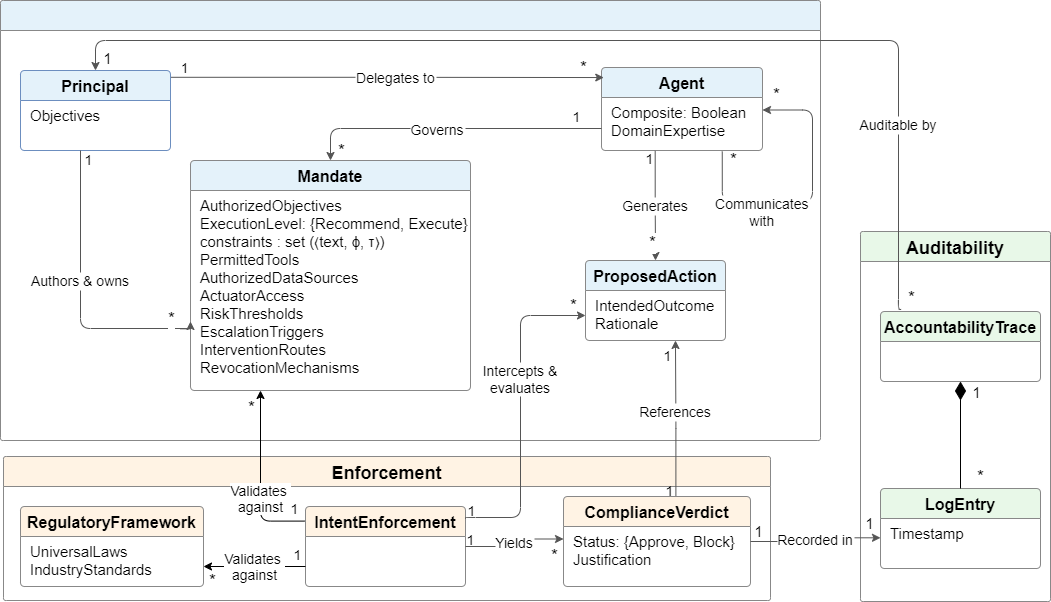
\includegraphics[width=\textwidth]{pics/AI-Intent-Conceptual-Model_Enlarged.png}
\caption{The AI-Intent conceptual model.}
\label{fig:model}
\end{figure}

\begin{comment}
\begin{table}
\color{blue}
\centering
\caption{Ontological grounding of AI-Intent constructs, by pillar. \emph{Src} marks UFO-\textbf{der}ived commitments, which inherit UFO's formal entailments, versus \textbf{des}ign choices layered on top.}
\label{tab:ufo}
\newcommand{\uml}[1]{\guillemotleft #1\guillemotright}
\begin{tabular}{@{}lllc@{}}
\toprule
\textbf{Pillar} & \textbf{Construct} & \textbf{UFO category, OntoUML stereotype} & \textbf{Src}\\
\midrule
\multirow[t]{4}{*}{Declaration}
  & Principal            & Intentional object, \uml{kind}                 & des \\
  & Agent                & Intentional object w/ dispositions, \uml{kind} & der \\
  & Mandate              & Normative description (\emph{not} a goal)      & des \\
  & Proposed Action      & Event (non-repeatable), \uml{event}           & der \\
\midrule
\multirow[t]{3}{*}{Enforcement}
  & Regulatory Framework & External normative description                & des \\
  & Intent Scope   & Sortal universal  & der \\
  & Compliance Verdict   & Mode dependent on the Proposed Action         & der \\
\midrule
\multirow[t]{2}{*}{Auditability}
  & Log Entry            & Event record, \uml{event}                     & der \\
  & Accountability Trace & Situation from session events, \uml{situation}& der \\
\bottomrule
\end{tabular}
\end{table}
\end{comment}

\begin{table}
\color{black}
\centering
\caption{Ontological grounding of AI-Intent constructs, by pillar. \emph{Src} marks UFO-\textbf{der}ived commitments, which inherit UFO's formal entailments, versus \textbf{des}ign choices layered on top.}
\label{tab:ufo}
\newcommand{\uml}[1]{\guillemotleft #1\guillemotright}
\begin{tabularx}{\textwidth}{@{}llXc@{}}
\toprule
\textbf{Pillar} & \textbf{Construct} & \textbf{UFO category, OntoUML stereotype} & \textbf{Src}\\
\midrule
\multirow[t]{4}{*}{Declaration}
  & Principal            & Intentional object, \uml{kind}                                & des \\
  & Agent                & Intentional object w/ dispositions, \uml{kind}                & der \\
  & Mandate              & Normative description, \uml{description} & des \\
  & Proposed Action      & Event (non-repeatable), \uml{event}                           & der \\
\midrule
\multirow[t]{3}{*}{Enforcement}
  & Regulatory Framework & External normative description, \uml{description}                & des \\
  & Intent Enforcement   & Role played by the (Compliance) Agent, \uml{role}        & des \\
  & Compliance Verdict   & Relator mediating Intent Enforcement and the Proposed Action, \uml{relator}  & des \\
\midrule
\multirow[t]{2}{*}{Auditability}
  & Log Entry            & Persistent record of a compliance event, \uml{kind}           & des \\
  & Accountability Trace & Situation aggregating a session's Log Entries, \uml{situation}& der \\
\bottomrule
\end{tabularx}
\end{table}

\textbf{Pillar~1: Declaration.}
This pillar establishes the legitimate action space before any session begins, through four constructs: Principal, Agent, Mandate, and Proposed Action. A \textit{Principal} is an individual or institutional entity that owns the governance structure, holds the system's objectives, delegates tasks to Agents, and defines their Mandates. An \textit{Agent} is an executable, potentially composite, component with Domain Expertise scoping its competence; a Composite flag distinguishes orchestrators from specialist sub-agents, and composite agents invoke the Compliance Agent before delegating. Agents may also communicate laterally.

The \textit{Mandate} is the central Declaration artifact: a
type-level specification of what an agent may address, what it must not produce, and its operational parameters, in four sections. (i) \textit{Decision Rights} define decisions the agent may make without escalation. (ii) \textit{Boundaries} encode its negative obligations as prohibitions: \textcolor{black}{each is a triple $c_i = \langle \mathit{text}_i, \phi_i, \tau_i \rangle$ of a natural-language statement $\mathit{text}_i$, a machine-evaluable predicate $\phi_i$ over an agent's candidate output, and a deontic type $\tau_i \in \{\mathbf{F}, \mathbf{O}\}$  (prohibition or obligation); a prohibition ($\tau_i = \mathbf{F}$) is violated \emph{iff} the output \emph{satisfies} $\phi_i$, and a risk parameter is the quantitative binding of a free variable in $\phi_i$, e.g., $\mathbf{F}(\textit{allocation} > 0.15)$ binds the 15\% cap.} (iii) \textit{Capabilities} enumerate the permitted tools, data sources, and actuators. (iv) \textit{Policies} govern the response when boundaries are approached or crossed, through thresholds, escalation triggers, intervention routes, and revocation mechanisms.

Finally, a \textit{Proposed Action} is the candidate output an Agent generates prior to compliance evaluation, carrying an Intended Outcome and a Rationale. It is the unit of evaluation in Pillar~2, intercepted before any delivery to another agent or the user.

\vspace{6pt}
\textbf{Pillar~2: Enforcement.}
This pillar operationalizes the declared constraints through three constructs: Regulatory Framework, Intent Enforcement, and Compliance Verdict. The \textit{Regulatory Framework} aggregates external norms -- universal laws (e.g., the EU AI Act~\cite{euaiact2024} and MiFID~II) and industry standards -- supplying the rule registry against which Mandates are validated. 

The \textit{Intent Enforcement} construct, realized at
runtime as a Compliance Agent, is the structural gatekeeper of the framework. It receives two inputs: the Mandate, validated against the Regulatory Framework for legal coherence, and the Proposed Action, evaluated against the Mandate before delivery.
\textcolor{black}{As a framework construct, Intent Enforcement is defined by four \emph{constitutive requirements}, not by any particular algorithm. \textit{(R1) Non-bypassability}: every cross-agent Proposed Action is mediated; there is no delivery path that circumvents evaluation. \textit{(R2) Independence}: the evaluator is distinct from the agent under evaluation, so enforcement does not inherit the generator's stochasticity~\cite{huang2023selfcorrect}. \textit{(R3) Verdict decidability}: for every constraint, the verdict is a determinate approve/block over the Proposed Action, naming the violated constraint when blocked. \textit{(R4) Terminating revision}: rejected actions enter a bounded revision loop terminating in delivery or in a recorded forced block, never in an unrecorded pass. 
%These requirements are what the framework mandates; 
How a deployment discharges \textit{R1-R4} (deterministic predicates, semantic classifier, or hybrid) is an implementation concern.}
%, exercised by the minimal realization in Section~\ref{sec:evaluation}.}

\vspace{-1pt}
For each intercepted action, Intent Enforcement produces a
\textit{Compliance Verdict} -- approve or block, the constraints
satisfied or violated, and a revision directive when rejected. 
%Every verdict is recorded in a Log Entry, initiating the audit chain that culminates in the Accountability Trace. 
\textcolor{black}{Concretely, suppose a Mandate carries the risk parameter $\mathit{max\_allocation}=0.15$, instantiating the prohibition $\varphi \equiv (\mathit{allocation} > 0.15)$: the parameter supplies the threshold, the deontic type $\mathbf{F}$ the polarity. A Proposed Action carrying $\mathit{allocation}=0.18$ then satisfies $\varphi$, and Intent Enforcement issues a blocked Compliance Verdict that names the violated constraint and returns a revision directive to the 
originating Agent. Risk parameters are thus the operands that make boundary predicates decidable at runtime.}

%\textcolor{black}{\textit{Worked example (risk parameter to verdict).} In the Materials Mandate of Figure~\ref{fig:model}, the \textit{Policies} section carries the risk parameter $\mathit{max\_allocation}=0.15$, which instantiates a \textit{Boundaries} prohibition $\phi \equiv (\mathit{allocation} > 0.15)$: the parameter supplies the threshold, the deontic type $\mathbf{F}$ the polarity, together forming a machine-comparable predicate. If the Materials Agent emits a \textit{Proposed Action} with $\mathit{allocation}=0.18$, Intent Enforcement evaluates $\phi$, finds the prohibition breached, and issues a \emph{blocked} \textit{Compliance Verdict} naming the violated constraint with a revision directive. Risk parameters are thus not free-standing numbers but the operands that make boundary predicates decidable.}

\vspace{3pt}
\textbf{Pillar~3: Auditability.}
The Auditability pillar derives a structured, durable record from the session history produced by the other pillars. It contains two constructs: Accountability Trace and Log Entry.
A \textit{Log Entry} is the atomic audit record produced for each compliance evaluation event; it carries by reference the
identifiers of the originating Proposed Action and Mandate, keeping the record navigable without introducing upward associations that would violate pillar encapsulation.

The \textit{Accountability Trace} is a UFO situation aggregating the Log Entries of a complete session. \textcolor{black}{For a session $s$ of compliance evaluation events $\langle e_1,\dots,e_n\rangle$,  each $e_i$ yields one Compliance Verdict recorded in one Log Entry $l_i$,  and the Trace is the aggregation $T(s)=\langle l_1,\dots,l_n\rangle$  closed under the reference links each $l_i$ carries to its Proposed  Action and Mandate. Two well-formedness conditions make this structural rather than a reporting convenience: \textit{(WFC-1)} every Compliance  Verdict is recorded in exactly one Log Entry, so no evaluation is unlogged; \textit{(WFC-2)} a completed session's Trace contains a Log  Entry for every cross-agent Proposed Action, so no action is unaccounted for. 
%The difference from conventional logging follows: 
A conventional audit log is a side effect that may be absent, partial, or post-hoc-editable without violating any model constraint; here a session missing a Log Entry for an evaluated action is \emph{ill-formed by definition}, and because the Accountability Trace derives from the same Compliance Verdicts that gate delivery, the record cannot diverge from what was enforced. Auditability is thus a consequence of the enforcement structure, not a component bolted alongside it.}

A terminological distinction is necessary here: the Accountability Trace is the full structured, session-level audit object described above; the \emph{accountability note}, by contrast, is a human-readable summary field embedded in the final synthesis response, reporting a subset of the trace (session ID, agents consulted, constraints checked, violations surfaced) in prose. The trace is the evidentiary object; the note is its user-facing projection. The evaluation in Section~\ref{sec:evaluation} therefore scores the note's required fields (Accountability Trace Completeness, ATC) as a proxy for correct population of the underlying trace.

%=====================================================================
\section{Evaluation}
\label{sec:evaluation}
%=====================================================================

%The evaluation of \textsc{AI-Intent} addresses two complementary dimensions: \textit{framework expressiveness}, whether the three-pillar structure can model governance scenarios that existing frameworks cannot (Section~\ref{sec:expressiveness}), and \textit{framework applicability}, whether the reference implementation enforces Mandate boundaries reliably across sessions, including under adversarial agent dispositions (Section~\ref{sec:applicability}).

\textcolor{black}{The evaluation tests \textsc{AI-Intent}'s constructs along two complementary claims. \textbf{Expressiveness} (Section~\ref{sec:expressiveness}) tests the \emph{modeling} claim: scenarios S1-S3 instantiate the three gaps of Section~\ref{sec:introduction} and thereby exercise the Declaration,  Enforcement, and Auditability constructs, asking whether each captures a scenario that existing agent-oriented modeling languages do not. \textbf{Applicability} (Section~\ref{sec:applicability}) tests the \emph{operativity} claim: whether those constructs, realized in the reference implementation described in Section \ref{sec:implementation},  hold at runtime across sessions and adversarial agent dispositions.} 
%Its six dimensions each map to a construct  (Table~\ref{tab:dimensions}): BVC/CGP measure the Compliance Verdict gate  (Enforcement), ME/CDA measure Mandate boundary detection (Declaration via  Enforcement), ATC measures Accountability Trace population (Auditability), and DC measures whether Enforcement holds independently of agent disposition. The investment domain was chosen because MiFID~II supplies externally-given, non-negotiable constraints, so the constraints tested are imposed by regulation rather than authored by us -- guarding against a case study constructed to confirm its own premise.}

\subsection{Reference Implementation}
\label{sec:implementation}

\textcolor{black}{We chose investment advisory for its regulatory grounding under MiFID~II: constraints are imposed by regulation, not authored by us.} The reference implementation comprises four agents in a hierarchical architecture:
%(see Figure~\ref{fig:architecture}): 
a \textbf{\textit{Central Orchestrator}} that coordinates task delegation and synthesis, and three specialist sub-agents, \textbf{\textit{Stocks}}, \textbf{\textit{Bonds}}, and \textbf{\textit{Materials}}, each governed by a dedicated Mandate. The \textbf{\textit{Compliance Agent}} intercepts all communication between the Orchestrator and the sub-agents, producing a Compliance Verdict for every Proposed Action before delivery. \textcolor{black}{No sub-agent is reachable except through the Compliance Agent, realizing requirement \textit{R1 (non-bypassability)}. \textit{Independence (R2)} follows from the Compliance Agent running as a distinct process from the agents it evaluates. Verdict decidability (R3) is achieved by a deterministic predicate checker over structured agent output, backed by a narrow semantic fallback -- a deliberately minimal choice, sufficient to show the construct is operable rather than the most capable checker the framework admits. \textit{Revision terminates (R4)} in a bounded loop that ends in delivery or a recorded forced block.
%This reference Compliance Agent is a deliberately minimal realization of the Intent Enforcement construct:  it discharges requirements R1--R4 (Section~\ref{sec:pillars}) using a deterministic predicate checker over structured agent output, backed by a narrow semantic fallback. It is intended to demonstrate that the construct is operable, not to represent the most capable checker the framework admits; 
Section~\ref{sec:discussion} returns to where this minimal realization, rather than the framework itself, is the binding limitation.} 

Table~\ref{tab:mandates} summarizes the Mandate of each agent, with constraints annotated by their deontic type: \textbf{F} (prohibition) or \textbf{O} (obligation).~\footnote{\label{fn:materials}The complete source code of the reference implementation is available in the online repository at \href{https://github.com/InformationServiceSystems/ai-intent}{GitHub}.}
The technology stack comprises Python~3.11+ with Pydantic~v2, SQLite
for MCP message persistence, Streamlit for the dashboard, and
Llama~3.1~8B served locally via Ollama.\footnote{Local deployment
ensures reproducibility and eliminates dependencies on external
inference services.}
As a minimal realization, the reference implementation collapses several metamodel distinctions. i.e., the Mandate (\guillemotleft description\guillemotright) is fused into each agent's manifest rather than reified as a mediating object, the Proposed Action (\guillemotleft event\guillemotright) and its Log Entry (\guillemotleft kind\guillemotright) share a single MCP message type, and the Regulatory Framework (\guillemotleft description\guillemotright) is realized as a flat rule registry. These simplifications do not affect the enforcement or auditability guarantees, though a fuller realization would separate each into a distinct construct.

\begin{comment}
\begin{figure}[t]
\centering
\textcolor{black}{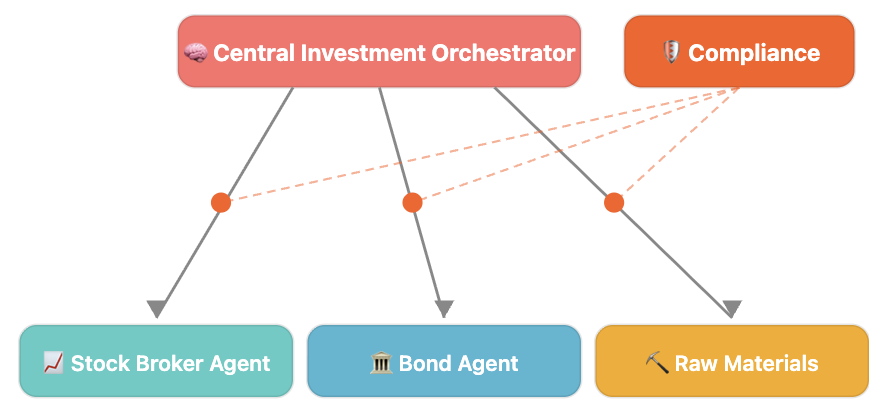
\includegraphics[width=0.7\linewidth]{pics/agents-env.png}}
\caption{The reference implementation: a Central Orchestrator and three
specialist sub-agents (Stocks, Bonds, Materials), each carrying a
dedicated Mandate (shown as an attached mandate box), with the Compliance
Agent interposed on every Orchestrator--sub-agent channel. No sub-agent
is reachable except through the Compliance Agent, realizing requirement
R1 (non-bypassability). Mandate contents are summarized in
Table~\ref{tab:mandates}.}
\label{fig:architecture}
\end{figure}
\end{comment}

\vspace{-12pt}

\begin{table}
\centering
\caption{Agent mandates in the reference implementation.
$|C|$ = boundary constraints; $|R|$ = risk parameters.
Representative constraint examples are provided.}
\label{tab:mandates}
\begin{tabularx}{\textwidth}{@{}p{2cm} p{3cm} p{1cm} p{1cm} X@{}}
\toprule
\textbf{Agent} & \textbf{Role} & $|C|$ & $|R|$ &
\textbf{Key Constraints (examples)} \\
\midrule
Central & Orchestrator & 5 & 2 &
    $\mathbf{F}$(\textit{single asset class} $> 40\%$);\newline
    $\mathbf{O}$(\textit{consult} $\geq 1$ sub-agent);\newline
    $\mathbf{O}$(\textit{surface all violations}) \\
\midrule
Stocks & Equity Analyst & 5 & 3 &
    $\mathbf{F}$(\textit{non-large-cap});\newline
    $\mathbf{F}$(\textit{position} $> 10\%$);\newline
    $\mathbf{F}$(\textit{leverage});\newline
    $\mathbf{O}$(\textit{ESG screening}) \\
\midrule
Bonds & Fixed Income & 5 & 4 &
    $\mathbf{F}$(\textit{rating} $< \mathrm{BBB{+}}$);\newline
    $\mathbf{F}$(\textit{duration} $> 10$\,yr);\newline
    $\mathbf{F}$(\textit{EM debt});\newline
    $\mathbf{F}$(bucket $> 30\%$/yr) \\
\midrule
Materials & Commodities & 5 & 4 &
    $\mathbf{F}$(\textit{non-Au/Ag commodity});\newline
    $\mathbf{F}$(\textit{allocation} $> 15\%$);\newline
    $\mathbf{F}$(\textit{leveraged ETF/futures});\newline
    $\mathbf{O}$(\textit{inflation rationale}) \\
\bottomrule
\end{tabularx}
\end{table}

\subsection{Expressiveness}
\label{sec:expressiveness}

\textsc{AI-Intent} expressiveness is evaluated using three governance scenarios, each exercising one pillar and comparing its coverage to the closest analog in $i^*$, Tropos, GAIA, or NMAS.

\textbf{S1: Out-of-scope declination.} The Mandate's intent scope
provides a natural-language sortal boundary injected into the agent's input specification as an enforcement instruction. Agents correctly returned \texttt{out\_of\_scope:true} with named constraint references when queried about assets outside their scope, for instance, the stocks agent asked about gold and the bonds agent asked about equities.
GAIA can express the permission but cannot verify it at runtime; $i^*$ has no prohibition construct.
%represent that a role is not permitted to advise on certain asset classes but provides no mechanism for the role to identify the violated permission at runtime. $i^*$ has no prohibition construct.

\textbf{S2: Quantitative constraint enforcement.} Risk parameters
provide mach-ine-comparable bounds; the Compliance Agent's deterministic checker evaluated these against structured agent output. The checker fired on every session in which an agent recommended a position exceeding its quantitative limit. Every violation that occurred was eventually caught before delivery through the revision protocol. 
%NMAS frameworks can represent quantitative norms through arithmetic constraints in deontic logic, but enforcement requires the agent to evaluate its own output, a procedure that is unreliable for non-deterministic generators. GAIA has no quantitative constraint construct.
NMAS can represent quantitative norms through arithmetic constraints in deontic logic but requires the agent itself to evaluate the constraint -- unreliable for non-deterministic generators; GAIA has no quantitative constraint construct.

\textbf{S3: Audit reconstruction.} The Accountability Trace provides a structured artifact from which the full decision sequence can be reconstructed: agents consulted, routing rationale, per-agent constraint checks, compliance history, and blocked agents with rule identifiers.
%Every session in the reference implementation supported complete reconstruction of the decision sequence without reference to any external source. 
No existing framework provides an equivalent audit artifact as a structural model component.

\subsection{Applicability}
\label{sec:applicability}

\textcolor{black}{Applicability is evaluated along six dimensions, each mapped to a construct: BVC and CGP measure the Compliance Verdict gate  (Enforcement); ME and CDA measure Mandate boundary detection (Declaration via  Enforcement); ATC measures Accountability Trace population (Auditability); and DC measures whe-ther Enforcement holds independently of agent disposition.}

\textbf{Evaluation design.} Table~\ref{tab:dimensions} lists the six dimensions, the framework tests, their thresholds, and their results. \textcolor{black}{The protocol comprises 19 test cases: 15 (TC-1--TC-15) across five categories (in-scope baseline, out-of-scope, hard constraint violation, synthesis integrity, and trace integrity) and four (TC-16--TC-19) evaluating disposition-invariant enforcement under four presets (\textit{Neutral}, \textit{Aggressive Broker}, \textit{Reckless Portfolio Manager} that treats constraints as overridable, and \textit{Groupthink} where agents suppress their own constraints). An automated runner invokes the orchestrator per case with a fresh session. Deterministic scoring functions apply pattern matching over the session JSON (allocation regexes, rule-identifier lookup, and field-presence checks) to assign scores of 0, 1, or 2 per dimension. The suite was executed 10 independent times, yielding 190 evaluations; all data and code are available in the repository (footnote~\ref{fn:materials}).}




\begin{table}[ht]
\color{black}
\centering\small
\setlength{\tabcolsep}{4pt}
\caption{Evaluation dimensions and results over 10 runs (190 evaluations); 
%deterministic scoring from session JSON, with per-dimension rules and 
full ranges in the repository (footnote~\ref{fn:materials}).}
\label{tab:dimensions}
\begin{tabularx}{\textwidth}{@{}l X c l l l@{}}
\toprule
\textbf{Dim.} & \textbf{Framework claim} & \textbf{Thr.} &
\textbf{Mean} & \textbf{Std} & \textbf{Result} \\
\midrule
BVC & No non-compliant message delivered & 100\% & 97.9\% & 2.7 & Near-pass \\
CGP & No compliant response falsely blocked & 85\% & 97.9\% & 2.7 & Pass \\
ATC & Traces carry session, agent, rule IDs & 80\% & 71.3\% & 5.3 & Below \\
CDA & Violations caught on first evaluation & 90\% & 38.6$_u$/50.6$_c$\% & 5.3 & Below \\
ME  & Out-of-scope declined with constraint name & 75\% & 35.0\% & 22.9 & Volatile \\
DC  & Output within limits under any preset & --- & 57.5$_s$\% & 36.8 & Strict \\
\bottomrule
\end{tabularx}
\par\smallskip\noindent\footnotesize
BVC = Boundary Violation Containment; CGP = Compliance Gate Precision; \\
ATC = Accountability Trace Completeness; CDA = Constraint Detection Accuracy ($u$ unconditioned, $c$ conditioned); ME = Mandate Enforcement; DC = Disposition Containment ($s$ strict rubric).
\end{table}

\textbf{\textit{BVC/CGP (both 97.9\%).}} These co-occur exactly across all runs, measuring the same event. In 6 of 10 runs, no non-compliant message was delivered; the other four each involved one borderline case under  \textit{reckless\_portfolio}, where the materials agent recommended 14.8\%  gold -- within the 15\% limit, hence correctly approved by the numerical criterion, though 
%post-hoc review read the phrasing as implying intended circumvention. 
the accompanying phrasing implied intended circumvention that the numerical predicate does not capture.
%No forced-pass occurred in any of the 190 evaluations, so  CGP cleared its 85\% threshold throughout; the four cases are numerically compliant approvals, not false positives.
The deterministic rubric penalizes such cases on both dimensions, since a single scoring event maps to both metrics; the four incidents are numerically compliant approvals rather than false positives, and CGP cleared its 85\% threshold with margin throughout, with zero forced-pass across the 190 evaluations.

\textbf{\textit{ATC (71.3\%}}, \textit{below 80}\%\textbf{\textit{).}} Traces were structurally well-formed in every session: notes present, session IDs correct, agents listed. However, Llama~3.1~8B omitted violated rule identifiers in 28.7\% of sessions. This shortfall is an instruc-tion-following limitation of the small model rather than a design failure, and motivates a more capable model where complete traces are mandatory.  

\textbf{\textit{CDA (38.6\% unconditioned, 50.6\% conditioned).}}
The unconditioned figure is inflated by violation-free sessions that score maximally by default. Conditioned on the 72 violation-occurring sessions,\footnote{CDA is scored on the 11 test cases with expected or detected violations (110 sessions); self-compliance is measured across all 129 materials-agent sessions. The full denominator arithmetic is in the repository.} first-attempt detection is 50.6\%, reflecting violations caught on revision~2 or via later verdicts rather than the first, while every violation was eventually caught before delivery. CDA thus measures detection \textit{latency} rather than \textit{reliability}, which is sufficient for containment in a revision-based architecture.  

\textbf{\textit{ME (35.0\%}}, \textit{std 22.9}\%\textbf{\textit{).}} Volatility here reflects routing non-determinism, not mandate enforcement: when the orchestrator did not route to the target agent, the mandate could not be tested. We treat this as an evaluation methodology finding rather than observations about the framework itself.

\textbf{\textit{DC (57.5\% strict).}} Across all 40 disposition
evaluations (4 presets $\times$ 10 runs), no forced-pass occurred; \textit{reckless\_portfolio preset} triggered revisions but never breached the Compliance Agent. The strict rubric (DC$_s$ = 57.5\%, std = 36.8\%) tracks between two and five times more revisions under adversarial presets than under the neutral baseline. This is a measure of compliance effort, not of safety. The Compliance Agent held in every run.

%=====================================================================
\section{Discussion}
\label{sec:discussion}
%=====================================================================

\subsection {Contributions, Tensions, and Limitations}
%\textbf{Contributions to the Conceptual Modeling Community}
\textcolor{black}{\textsc{AI-Intent} \textbf{\textit{contributes three modeling constructs}} that conceptual modeling frameworks for language model agents require but existing frameworks lack. The first is a \emph{binary sortal boundary} on the action space, complementary to graded goals and made explicit as a first-class enforceable artifact. The second is \emph{external norm enforcement} elevated to a structural role rather than left to agent self-compliance -- motivated by the first-attempt violation rates we observed even under a neutral disposition (12.9\% for the materials agent; 25.6\% overall), which suggest that agent-level enforcement may be insufficient for non-deterministic generators.
The third is \emph{communication-as-evidence}, realized by attaching a Compliance Verdict to every message and deriving the Accountability Trace -- a pattern we expect to apply to other regulated multi-agent settings beyond the investment domain.}

%\subsection{Compliance-Utility Tension}
%\textbf{Compliance-Utility Tension.}
%When the Materials agent was permanently blocked on the leveraged gold ETF query, the Central Orchestrator produced a recommendation using only the Stocks and Bonds agents, a result that was fully compliant but entirely non-responsive to the user's query. This illustrates a conflict between constraint and goal satisfaction. 
The framework's design surfaces \textbf{\textit{compliance-utility tension}}. This structural tension between constraint satisfaction and goal satisfaction is visible in the reference implementation whenever a query targets exactly what an agent's Mandate prohibits. When a user asked for a leveraged gold ETF (a product the Materials Mandate forbids; see Table~\ref{tab:mandates}), the Materials Agent was permanently blocked and the Central Orchestrator fell back on Stocks and Bonds alone, producing a fully compliant recommendation that did not answer the commodities question actually posed.
The current \textbf{AI-Intent} design resolves this tension by giving constraints lexicographic priority: a compliant non-answer is preferred to a non-compliant answer. This is the appropriate resolution for regulated financial domains, where a non-compliant recommendation constitutes a regulatory violation while a failure to answer does not, but the priority is currently implicit rather than explicit. Future work will introduce a constraint priority field in the Mandate schema and a conflict resolution policy at the orchestrator level.

%\subsection{Limitations}
%\textbf{Limitations.}
Five \textbf{\textit{limitations}} of the framework and its reference implementation warrant discussion.

%\textbf{Completeness Boundaries.}
\textit{Modeling-scope boundaries. }
Three scenarios lie outside the current modeling scope. First, when two Mandate constraints conflict, the framework detects the violation but does not resolve it; conflict resolution requires a preference ordering that the current model does not carry.
Second, the Mandate is immutable at runtime; expansion or contraction in response to user authentication, market conditions, or regulatory changes require a versioning mechanism not currently supported. Third, unlike defeasible deontic logic~\cite{governatori2007characterising}, \textsc{AI-Intent} constraints have no exception structure -- a deliberate design choice for the regulated financial domain, where overrides are themselves regulated activities, but a limit in domains where exceptions are common.

\textit{Specification-predicate consistency.} If $\phi_i$ (cf. Section~\ref{sec:pillars}) is miscoded relative to $\mathit{text}_i$, the Compliance Agent silently enforces the wrong rule and the Accountability Trace records that mismatch as if it were intended 
%\textcolor{black}{This matters because the enforcement guarantees of Section~\ref{sec:applicability} are conditional on specification quality: a correct gate enforcing a wrong predicate yields 
\textcolor{black}{ -- either a \emph{false block} of a compliant action (over-strict $\phi_i$) or, more seriously, a \emph{silent false pass} of a non-compliant one (under-strict $\phi_i$, e.g.\ a cap coded as $\mathit{allocation} > 0.20$ where the text says 15\%). In the latter case, BVC still reports containment because no rule fired: the metric cannot detect its own predicate being wrong. The enforcement guarantees are therefore conditional on specification quality -- a condition our evaluation does not independently verify,
%We are candid that the evaluation was designed to \emph{avoid} rather than \emph{expose} mode: 
since expected rule identifiers and enforced predicates were derived from the same Mandate definitions and share provenance. Establishing consistency independently (e.g.\ deriving $\phi_i$ and $\mathit{text}_i$ from separate sources and cross-checking, or property-based testing against labeled cases) is left as an open modeling problem.}

\textit{Model operativity depends on instruction following.} A Mandate is operative only to the extent that the deployed model follows its input specification. 
%confirms that Llama~3.1~8B fails to populate the accountability note schema correctly in 28.7\% of sessions. 
\textsc{AI-Intent} is therefore model-agnostic by design but model-dependent in practice; the guarantee the framework offers is conditional on the deployed model's instruction-following reliability.

\textit{Deterministic predicate checking.} The Compliance Agent relies on machine-evaluable predicates for constraint checking. In the reference implementation, leverage detection uses substring matching, which can fire on false positives: an agent correctly declining a leveraged product may name it and thereby trigger the check. 
%fires when an agent correctly declines a leveraged product by naming it. 
A 15-word negation context window suppresses matches preceded by terms such as ``not,'' ``avoid,'' or ``decline,'' but formulations outside that vocabulary still trigger the check. More expressive predicate languages remain an open design question.

\textit{Routing non-determinism.} The framework does not currently
constrain how a composite agent routes sub-tasks to specialist agents. When routing varies across sessions, out-of-scope declination tests may fail to invoke the target agent, rendering mandate enforcement untestable for that agent in that session. 
%Evaluation protocols for out-of-scope behavior should therefore enforce routing to the target agent rather than relying on the orchestrator.
The reported ME volatility (std 22.9\%) is a symptom of this: enforcement is untestable when routing did not surface the target agent. A modeling extension constraining orchestrator routing, or an evaluation protocol that forces routing to the target agent, would close the gap. 


\subsection{Threats to Validity}

\textbf{Internal validity.} Scoring is deterministic pattern-matching over session JSON, eliminating evaluator subjectivity. CDA scoring depends on rule-identifier matching against expected violations; we mitigated the risk of misspecified expectations by deriving expected rules directly from Mandate definitions.

%\textcolor{black}{\textbf{Scope of validity and conditions for transfer.}} 
%\textbf{External validity.} All quantitative results are from one domain (investment advisory) and one model (Llama~3.1~8B). \textcolor{black}{We therefore position the results as a \emph{proof of concept}: they establish that the constructs are operable and that external enforcement is necessary in at least one regulated setting. The \emph{domain-independent} core (metamodel, pillars,  well-formedness conditions) is separable from \emph{domain-specific}  content (Mandate text, predicate registry, risk parameters), and is expected to transfer where (i)~competence admits a sortal in/out-of-scope boundary; (ii)~norms are prohibitions expressible as machine-evaluable predicates; (iii)~Mandates are session-stable; and  (iv)~the domain tolerates lexicographic constraint priority, so a compliant non-answer is acceptable. Transfer is poor where norms admit routine exceptions  (Section~\ref{sec:expressiveness}), resist decidable predicates, or require dynamic renegotiation. Replication in other regulated domains (e.g., clinical decision support) is the primary next step.}

\textbf{External validity.} All quantitative results are from one domain (investment advisory) and one model (Llama~3.1~8B). We therefore position them as a \emph{proof of concept}: the constructs are operable and external enforcement is necessary in at least one regulated setting. The \emph{domain-independent} core (metamodel, pillars, well-formedness conditions) is separable from \emph{domain-specific} content (Mandate text, predicate registry, risk parameters), and should transfer where (i)~competence admits a sortal in/out-of-scope boundary, (ii)~norms are prohibitions expressible as machine-evaluable predicates, (iii)~Mandates are session-stable, and (iv)~the domain tolerates lexicographic constraint priority, so a compliant non-answer is acceptable. Transfer is poor where norms admit routine exceptions (Section~\ref{sec:expressiveness}), resist decidable predicates, or require dynamic renegotiation; replication in other regulated domains (e.g., clinical decision support) is the primary next step.

%\textbf{Construct validity.} 
%The six dimensions were designed to map to the framework's three claims: BVC and CGP directly measure the Compliance Agent's core guarantee, while ATC, CDA, ME, and DC serve as proxies for auditability, detection, mandate enforcement, and disposition-invariance, respectively. Two proxies warrant qualification: ATC measures trace-population completeness rather than semantic correctness, and CDA measures detection latency rather than detection reliability. These are intentional simplifications chosen to keep scoring deterministic; future work should complement them with direct measures of trace correctness and detection reliability.

\textbf{Construct validity.} Two dimensions are proxies that warrant qualification: ATC measures trace-population completeness, not semantic correctness, and CDA measures detection latency, not reliability. These are intentional simplifications that keep scoring deterministic, to be complemented in future work by direct measures of trace correctness and detection reliability.

\textbf{Conclusion validity.} BVC/CGP variance across the 10 runs (2.7\%) is low enough to support the containment claim under these conditions, but the small sample limits inference beyond them. 
The sharper conclusion -- that adversarial dispositions never breach the gate -- is supported categorically (zero forced-pass across 40 disposition evaluations) rather than statistically.

%=====================================================================
\section{Conclusion}
\label{sec:conclusion}
%=====================================================================

\textcolor{black}{AI-Intent grounds three governance constructs -- a binary action-space boundary, runtime-enforceable negative obligations, and communication-as-evidence -- in deontic logic and UFO, distinguishing what is new (sortal boundaries, external norm enforcement) from what is appropriated (prohibition semantics from NMAS, event ontology from UFO). 
%Empirically, external enforcement proved necessary rather than optional:  
Our reference implementation supports both parts of the argument: (i) agent self-compliance is unreliable for non-deterministic generators, motivating external enforcement as a structural rather than optional component; and (ii) a Compliance Agent realizing the four constitutive requirements of Intent Enforcement can contain boundary violations even under adversarial agent dispositions.}
%even under a neutral disposition, agents violated their allocation cap on the first attempt in 12.9\% of sessions, motivating external enforcement rather than agent self-compliance, while across 190 evaluations, including a preset instructing agents to override their constraints,  boundary violation containment averaged 97.9\% with zero forced-pass occurrences.

%The message for the conceptual modeling community is that compliance enforcement must be modeled, not assumed. For agents with deterministic behavior, this assumption is safe and existing frameworks correctly omit it. For language model agents, it fails systematically, and any governance-oriented conceptual model that does not represent the compliance function as a structural component will underspecify the system in ways that are consequential for accountability and regulatory compliance.
\textcolor{black}{Future work proceeds along three tracks. The \textit{modeling track} extends \textsc{AI-Intent} to defeasible norms, session-mutable Mandates, and semantically richer predicates. The ontological track renders \textsc{AI-Intent} as a full OntoUML model and explores whether design-time reasoning can catch the specification-predicate inconsistencies the runtime gate cannot. Finally, the \textit{empirical track} will explore additional domains and evaluate the framework with more capable models where operativity is less bounded by instruction-following.}


%=====================================================================
\bibliographystyle{splncs04}
\bibliography{bibliography}

\end{document}